%\affiliation{\affilnum{1}Dept. of Computer Architecture and Computer Technology, University of Granada, Spain}

%\corrauth{Pablo Garc\'ia-S\'anchez,
%ETS. Ingenier\'ias en Inform\'atica y Telecomunicaci\'on and CITIC-UGR,
%C/Periodista Daniel Saucedo s/n,
%Universidad de Granada,
%18071, Granada, Spain.}

\documentclass[preprint]{elsarticle}
\usepackage[latin1]{inputenc}
\usepackage[english]{babel}
\usepackage{moreverb,url,color}
\usepackage{algorithm}
\usepackage{algorithmic}
\usepackage{graphicx}
\usepackage{color}
\usepackage{url}
\usepackage[colorlinks,bookmarksopen,bookmarksnumbered,citecolor=red,urlcolor=red]{hyperref}

\begin{document}

\begin{frontmatter}

%%%%%%%%%%%%%%%%%%%%%%%%%%%%%%%   TITLE   %%%%%%%%%%%%%%%%%%%%%%%%%%%%%%%
\journal{Applied Soft Computing}
\title{Distributed multi-objective evolutionary optimization using island-based selective operator application}

%%%%%%%%%%%%%%%%%%%%%%%%%%%%%%%   AUTHORS   %%%%%%%%%%%%%%%%%%%%%%%%%%%%%%%

\author{P. Garc\'ia-S\'anchez$^1$, J. Ortega$^2$, J. Gonz\'alez$^2$, P. A. Castillo$^2$ and J.J. Merelo$^2$}
\ead{pablo.garciasanchez@uca.es, \{jortega, jesusgonzalez, pacv, jmerelo\}@ugr.es}
\address{
$^1$ Department of Computer Science and Engineering. ESI. University of C\'adiz, Spain\\
$^2$ Department of Computer Architecture and Computer Technology.\\ ETSIIT - CITIC. University of Granada, Spain\\
}


\begin{abstract}
  % First, state the problem!!!! - JJ Pablo: ok!
%Real-world optimization problems usually require to deal with several objectives.
%Multi-objective optimization methods have gained interest in the last
%years because of the performance they can achieve solving this kind of problems. 
%Many of them usually require a high-dimensional
%decision space, and multi-objective Evolutionary Algorithms have been
%successfully used in the past. Due to the large computational cost
%these algorithms require, different parallelization and distribution
%methods have been proposed, with different parallel and distributed
%computer architectures to cope with them. 

  \textcolor{blue}{Real world optimization problems usually have many dimensions and
  several objectives. The high dimensionality requires exceptional
  computing power, and the fact that several dimensions have to be
  searched at the same time add additional difficulty.}
% One of the most extended methods to deal with high-dimensional
% multi-objective optimization problems are the distributed
% co-evolutionary algorithms.
% ----------------- This sentence is meaningless. It should be
% substituted by other stating that co-evolutionary algorithms can
% deal with it for some reason
% Besides, we're no longer saying that they are co-evolutionary in the
% title, but "island-based selective operator application". This
% should go to the abstract too - JJ
  
In these methods %which ones? coevolutionary or selective operator
                   %application? - JJ
  each processor deals only with a part of the decision
space, that is, the individuals belonging to the same sub-population,
\textcolor{blue}{which are called {\em islands} in this context}, explore the same subset of decision variables. However, only
decomposable problems could be strictly implemented in parallel this
way. \textcolor{blue}{A new approach, which we call {\em selective operator application} is presented here to deal with un-decomposable
problems:} % so we are saying that high-dimensional multi-objective
          % problems are a challenge, but we are presenting a solution
          % for non-decomposable problems. What's what? - JJ
instead of sharing parts
of individuals, each processor applies the variation operators to a
specific subset of the whole individual. % this solves... - JJ
We have previously proved
that extending the length of these subsets, and therefore, sharing
\textcolor{blue}{some search space between islands, implies an improvement in different performance metrics}.
 % which results? - JJ PABLO: answered
But in this paper, a new method to automatically
adapt the size of the overlapping, or shared sections, of the
individuals has been compared to other collaborative evolutionary
techniques considering different number of islands, chromosome sizes
and benchmarks. The analysis of the obtained experimental results, by
using different metrics, shows that our approach can provide
statistically significant improvements with respect to the base
algorithm \textcolor{blue}{in high-dimensional multi-objective problems}. % in high-dimensional multi-objective problems? - JJ PABLO: ok, puesto
Results also show that the relation between the number of
islands (subpopulations) and the length of the chromosome (number of
decision variables) is also a relevant factor to determine the most
efficient alternative to distribute the decision variables.  
\textcolor{blue}{This opens up a new challenge that can be addressed in the future.}
% This
                                % solves a problem or challenge we
                                % hadn't stated. - JJ Pablo: metido, mira a ver si queda frase memorable


\end{abstract}


\begin{keyword}
Multi-objective algorithms \sep NSGA-II  \sep distributed evolutionary algorithms \sep Island model
\end{keyword}

\end{frontmatter}





\section{Introduction}

%Introduction should start in the same way as the abstract. And
%starting with something that is not really applicable here, talking
%about general parallel evolutionary algorithms, is even worse.
% Right way (IMNSHO)
% 1. Multiobjective problems are
% 2. They usually require a good amount of computation → parallel
% distributed
% 3. One way to solve them is to use MOEAs _because_ they can be
% easily parallelized
% 4. But the easy paralellization is not necessarily efficient.
% 5. We have proposed the HPMOON (or whatever) technique to improve
% it. In paper (whatever) we proved that (whatever)
% 6. In this paper we will be proving whatever - JJ FERGU: Addressing JJ order
% OK - JJ

%1. MOP ARE
Multi-objective optimization problems (MOP) are those where several
objectives have to be simultaneously optimized
\citep{Mora13paretobased,LIU2017344}. Solving a MOP implies optimizing a function composed of several independent cost functions, one per objective. In
these problems the aim is to obtain a set of solutions that are better
than the rest, considering all the objectives; this set is known as
the Pareto Front (PF). The solutions in this set are {\em non-dominated},
which means that there is no other solution that is equal or better
for all objectives; the objective of MOP algorithms is to find as many
solutions in the Pareto Front as possible, and in order to do that the
exploration of the search space must be very efficient, trying to
cover many possible exploration paths at the same time. 

%2 COMPUTATION -> PARALLEL
This aspect of searching for non-dominated solutions, as well as, in
many cases, the size of the search space itself, implies a high demand
of computational time, leading to the proposal of parallel and distributed methods to solve them
\citep{Luna15Survey,Mukhopadhyay14Survey,Chavez15MO,Hidalgo16residualstress,KAUR2018183,XU2018268},
%3 ONE WAY IS TO USE MOEAS BECAUSE
one of which are evolutionary algorithms (EAs)
\citep{DBLP:series/ncs/EibenS15}. EAs are bio-inspired meta-heuristics
that can be effectively used to find nearly optimal solutions for
optimization problems and are easily paralellizable, since they are
population-based and creating a functionally equivalent parallel
version is as easy as distributing the population in communicating
computing nodes, which are usually called islands. The fact that
they are population-based helps find many solutions that compose the
Pareto fron simultaneously.

Usually an EA starts by generating a set of random solutions, called
\emph{population}, following a user-defined description. Then, it
evaluates each candidate solution, called \emph{individual}, assigning
it a \emph{fitness} value, that describes how good the individual is
with regard to the target problem. New solutions are then generated by
the application of \emph{operators} that either mutate a single
solution or recombine different existing solutions. After each
iteration, called \emph{generation}, the least fit individuals are
removed, and the process continues until a user-defined stop condition
is met.

One of the best known and referenced MOEAs
\citep{Dorronsoro13superlinear} is the {\em 
  Non-dominated Sorting Genetic Algorithm} (NSGA-II)
\citep{Deb00NSGAII}. Classical genetic operators are applied to all
the individuals, which are divided into different ranks, based on the
dominance, to be selected for the next generations. 
% This paragraph has nothing to do with anything. Is it useful for
% what you are doing in the paper? Is there any challenge that you
% will be solving here? For instance, you could talk about the problem
% it's got for parallelization and how it deals with them - JJ

%4 BUT THE EASY PARALLELIZATION IS NOT NECESSARILY EFFICIENT

Different approaches have been used to parallelize EAs, as each individual can be considered as an
independent unit \citep{Alba13parallel}. Classic methods, such as the
global parallel EAs (Master-Slave), or the spatially structured
algorithms (Island model or Cellular EAs) have been applied
successfully in the past \citep{Folino03cellular,Alba02Parallelism}.
However, in the case of MOEAs, these
approaches \citep{Luna15Survey} need to deal with the whole solution set, the PF.
 This implies to use different distribution
and sharing mechanisms, as there exist a tradeoff between the speedup
achievable from parallelization and the need to globally recombine the
results to accurately identify the PF
\citep{Branke04Parallelizingcone}. % Is that the case with NSGA? - JJ

MOPs usually require a high number of variables, % No they don't, and
                                % if they do, add a reference - JJ
meaning that the
MOEAs need to deal with large individuals and spend significant extra
time for crossover, mutation and migration. %depending on the
                                %language, this time might not be
                                %significant at all, and will depend
                                %on the length of the chromosome, not
                                %the part of the chromosome you will
                                %be applying it to. Besides, this is
                                %not the critical part of the
                                %algorithm, the critical part is
                                %searching the solution space. 
Different authors have % this is only one possibility. You should talk
                       % about simple island models, too - JJ
proposed methods to divide the decision space (the chromosome) to
improve the performance and solution quality. In this aspect, the
co-evolution model is a dimension-distributed model where a % first
                                % reference to co-evolution in this
                                % paper. Is it still a paper about
                                % co-evolution? - JJ
high-dimensional problem is divided into lower dimensional ones
\citep{Gong15models,Tonda12cooperative}, and evolved separately. One
example of application of this technique was described in
\citep{Kimovski15Parallel}. The method presented in that work involves
different workers that evolve sub-populations created and recombined
by a master process, which performs different recombination
alternatives from the parts returned by worker processes. A high
dimensional problem was used to compare these 
alternatives. In \citep{Dorronsoro13superlinear}, a distributed
co-evolutionary island model was used.  Although in both papers
significant speedups were attained, only a low number of nodes were
employed (8). However, when the number of islands is increased, the division
of each section of the chromosome becomes smaller, and the scalability
may be affected by obtaining lower quality solutions in the same
amount of time. 





%5 WE HAVE PROPOSED HPMOON



A similar approach used to solve this kind of problems is the {\em
  selective operator application} (SLA). In this case, each island
deals with the whole chromosome, but only modifies a fragment of it in
the crossover and mutation phase depending on the number of islands,
using the whole chromosome for fitness calculation. This allows to
deal with un-decomposable problems. % if the whole chromosome is used,
                                % mutation and crossover will take the
                                % same time. You are modifying the
                                % search space, though. 
In our previous work \citep{Garcia16hpmoon} we used this method in a
preliminary experimental setup, although it is worth mentioning we are
establishing its name and acronym in this paper for the first time.
We proved 
that applying the variation operators only over specific sections of the whole chromosome improves the quality of the solutions in the same computing time for a multi-objective island-based algorithm.
Moreover, instead of making every island focus on a disjoint subset of the
chromosome, the usage of overlapped (shared) sections of the
chromosome 
can improve the quality of the solutions 
when the number of islands is increased. On that paper we proved that the most
adequate overlapping size may vary depending on a relation between the
number of islands and the individual size. However, it was a proof-of-concept, and the experiments
were conducted in a limited experimental system: mono-processor and
synchronous island model. %where we couldn't prove that... Or, we
                          %couldn't experiment... - JJ
This
motivates us to continue this research line using a more complete environment: a real cluster with up to 128 nodes, and a more complete parameter setting. Besides comparing previous methods in this new experimental setup, in this paper we propose
a new method that automatically adapts the size of the overlapped
sections depending on the number of available islands, comparing it with previous versions. 
% We have to
                                % emphasize what is actually done. Is
                                % this an addition to the old paper,
                                % or a complete rewrite? - JJ FERGU: rewritten previous paragraph


%6 IN THIS PAPER WE WILL BE PROVING

The hypothesis of this paper is that the use of automatically calculated overlapped sections of the
chromosome for the SLA can improve the
quality of the solutions in the same computing time with respect to
the baseline, disjoint and partly overlapped methods. 
These overlapped sections are calculated from the number of available islands, in a
multi-objective island-based algorithm, and tested in a real computational environment.

In order to prove this claim, our new automatic method has been
compared against different overlapping island schemes: a
baseline version of a distributed NSGA-II \citep{Deb00NSGAII}, a
SLA version with disjoint sections and a SLA
fixed-size overlapped version. 
Several benchmark problems and different large number of islands
have been used. Results show that this new technique can improve
different quality indicators in the same amount of time when the
problem size is large.  

The rest of the paper is organized as follows: after the State of the Art in distributed and co-evolutionary MOEAs, 
the used methodology and the compared algorithms are described in Section \ref{sec:methodology}. 
Then, the results of the experiments are presented (Section \ref{sec:results}), Finally, the conclusions and future work are discussed.


%%%%%%%%%%%%%%%%%%%%%%%%%%%%%%  STATE OF THE ART  %%%%%%%%%%%%%%%%%%%%%%%%%%%%%
%
\section{State of the Art}
\label{sec:soa}




% Parallel multiobjective optimization is the theme. And there are
% papers that do that. Please include them in the state of the art:
% dennis2003parallel (added to bibliography). FERGU: why this paper in particular? It parallelizes the fitness function steps and it is not multi-objective. It does not even describes the GA in detail.

Since the early 2000s distributed and parallel EAs
 have been used mostly to leverage systems such
as clusters or grids \citep{Talbi08Parallel}, since a first-order
approach to EA parallelization is as easy as dividing the population
and add a simple communication mechanism among them. But in the case of
MOEAs, the distribution and parallelization is not as direct as in
single-objective EAs. This is because in different steps of the
algorithm a whole set of dependent solutions, the Pareto Front, should
be managed as a whole, spending time in gathering all individuals from
the different processors or islands. 

To solve this issue, some authors have proposed using Master-Slave approaches. For example,  \citep{Durillo08masterslave} compared different master-slave approaches: synchronous generational, asynchronous generational and asynchronous steady-state, being the latter the most promising option. On the other hand, the method proposed by Hiroyasu \citep{Hiroyasu07discussion} generates offspring depending on the computational power.

%This is an improvement over the previous? What is the relationship? FERGU: linked
Other kind of approaches have also been explored. The work by Deb et al. \citep{Deb03distributed} was one of the first approaches for distributed MOEAs (dMOEAs). In that work, the dominance of the solutions was divided into the islands using a coordinate transformation. In that paper, authors concluded that dividing the search space is a good idea, although achieving this is not trivial. The division of the search space has been explored by other researchers, for example, dividing the population in elite and search sub-populations \citep{Wang09parallel}, or separating it in processors by objective \citep{Xiao03specialized}. \textcolor{blue}{For example, in \cite{Zhang17DECAL}, a weighted function is used to decompose the objective function and every subpopulation is responsible to solve the problem defined by a weighted vector.} Other authors, such as Martens \citep{Martens13asynchronous} use migration to accept individuals based on diversity, and migrating from not-crowded areas.

% Is this really cooperative co-evolution? - JJ FERGU: You mean the Dorronsoro one? The title says it
\textcolor{blue}{Many real-world problems require high-dimensionality \cite{Zhang17DECAL,XU2018268}.
Addressing this kind of problems with cooperative co-evolution has
also been studied in several works with approaches closer to the one
presented here.} The approach to focus on a portion of the chromosome,
as in our overlapped method, was firstly used in the work by
Dorronsoro et al. \citep{Dorronsoro13superlinear}, obtaining
super-linear performance 
in several instances. \textcolor{blue}{Recently, this approach has also been tested using a Particle Swarm Optimization (PSO) algorithm \cite{DorronsoroPSO2018}, also obtaining significant improvements in speedups and solution quality}. 

The approach described by Dorronsoro et al. has also been used by Kimovski et al. \citep{Kimovski15Parallel}, but using a
master-slave method that splits the population into several processors. As in previous works, each node
runs a parallel MOEA that only affects some portion of 
the individuals and the master
process receives all the sub-populations to be combined every certain number of generations. Up to 8 processors
were used in the experimental setup, and several
combination alternatives were compared. The main difference of our work with respect to previous works is that our approach does not 
broadcast all solutions to all islands for recombination, but only one solution to a random island, needing less
communication time. Moreover, Dorronsoro or Kimovsky approaches limited the maximum number of islands to 8, while in this paper we have
used up to 128 islands. 

Giving the responsibility of different parts of the search space to
different modules, has also been explored lately by some
researchers. For example, some authors focus on the solution space
modeling the PF by dividing it in different clusters, allowing an
easily parallelizable {\em divide and conquer} approach
\citep{cheng2015adaptive}. 
Even other types of metaheuristics, 
such as the Multi-Objective Ant Colony Optimization (MOACO) 
or Artificial Bee Colony Algorithm, 
can rely on island models to divide the search space depending on 
the node to achieve better results \cite{Mora13paretobased,LUO2017235}. 

In our previous work \citep{Garcia16hpmoon} we used some of
the aforementioned ideas to compare two different dMOEAs. The first
one divided the chromosome into $P$ sections, being $P$ the number of
islands. Every island $p$ only performed the mutation and crossover in
that part ($p_{th}$) of the chromosome (the selective operator application), while the fitness was
calculated using the whole individual. After a certain number of
generations, individuals were migrated randomly to other islands. The
performance metrics were calculated at the end of the run. The second
method, selective operator application with overlapping islands, used the $p_{th-1}$ and
$p_{th+1}$ sections of each chromosome, besides the $p_{th}$
part. During the same amount of time both methods obtained better
results than a baseline algorithm that dealt with the whole chromosome
in each island for crossover and mutation. We discovered that the
performance using one or another method depends on the number of
sections of the individuals and the number of islands used. This
motivated us to find a new automatic method to select this number of
sections of the chromosome to use, depending on the number of
islands. Besides, previous experiments were performed on a single
processor synchronous island model with a limited number of islands
(8, 32 and 128). In this paper,  8, 16, 32, 64 and 128 islands have
been used, and on this occasion, the experiments have been run on a parallel
cluster. Therefore, at the same time we are proposing an automatic
method to divide the individual search space, and also validating the
previous approach. 


We will describe how we have tested our approach in the next Section.




%
%%%%%%%%%%%%%%%%%%%%%%%%%%%%%%  METHODOLOGY  %%%%%%%%%%%%%%%%%%%%%%%%%%%%%
%

\section{Methodology} % This should be called
                                % methodology. The object of the
                                % section is to explain the
                                % methodology used to test the
                                % problem, in order to do that we have
                                % tested different versions that prove
                                % that our methodology works for the
                                % precise reasons we think it works- JJ FERGU: Done, and explained
\label{sec:methodology}

The objective of this section is to explain the methodology we have followed to
compare the different versions of the overlapping schemes.

\subsection{Proposed methods}
In this paper we analyse several SLA algorithms we have
implemented by using a parallel multi-objective baseline algorithm
as a basis for comparisons. Our proposed methods, using different overlapping schemes, %methods or method?
                                %Which methods? - JJ Fergu: clarifying
are based on NSGA-II, as almost all the previous works discussed
before
\cite{Dorronsoro13superlinear,Durillo08masterslave,Hiroyasu07discussion,Deb03distributed,Xiao03specialized,Wang09parallel,Martens13asynchronous}. % This is SoA stuff - JJ FERGU: Yes, I added it here againg because a reviewer wasn't very attentive
Therefore, we have used a basic distributed NSGA-II algorithm without
overlapping sections as the baseline (B).

%This probably should deserve a "Algorithm" environment too - JJ FERGU: You mean the LaTeX one? I've used it in the pseudocode figures
This basic distributed algorithm spreads the population among $P$
islands; after a fixed number of generations,
one individual in a given island is migrated to another random island,
thus avoiding to synchronize the global PF every
certain number of generations as other methods described in Section 2
do. At the end of the run, the PFs of all islands are
aggregated into a new one, and the quality measures are evaluated. 
Different  SLA alternatives can be devised to evolve the
subpopulations according to the decision space to be explored by each
island. Here we will consider three methods in which each island only
performs crossover and mutation in specific sections of the
individuals. 



%This algorithm is a regular NSGA-II algorithm distributed along a number $P$ of islands. After a fixed number of generations, one individual is migrated to another random island. At the end of the run, PFs of all islands are aggregated in a new one in order to compute the quality measures. This baseline method has been chosen as it does not require synchronization of the global PF every certain number of generations, as other methods described in Section 2 do.
%% some justification on why this was chosen - JJ PABLO: Added 
%
%% And some liaison to next subsection - JJ
%This method will be compared to different co-evolutionary approaches that are similar to the baseline, with the exception on the decision space to explore in each island.
%Three different co-evolutionary methods have been used. In all these methods, each island only performs crossover and mutation in specific sections of the individuals.

As in the baseline (B), an individual is migrated to another random
island after a fixed number of generations. In the new island, this
individual will be considered as one of the others in the island,
crossed and mutated in the same way, depending on the island
identifier (from 1 to $P$). Note that, differently from other works such as the ones
described by Talbi et al. \citep{Talbi08Parallel}, all the islands deal
with complete chromosomes for fitness calculation, so our approach can
deal with decomposable and no decomposable problems. %Don't understand what you say
                                %here. What you are saying is that our
                                %approach can't deal with decomposable
                                %problems, actually. - JJ FERGU: you are right, fixed

The methods we have tested are presented in the next subsections. 

\subsubsection{SLA with disjoint islands (D)} 
In this approach, each individual of size $L$ is split into $P$ chunks
of size $L/P$. Every island $p$ only performs crossover and mutation
on the $p_{th}$ part of the individuals. Figure \ref{fig:disjoint}
describes this approach.
%
\begin{figure*}[h!tb]
\centering
\includegraphics[width=12cm]{islandDisjoint.jpg}
\caption{SLA with disjoint islands (D): every island $p$ only modifies the $p_{th}$ components (in grey) of the individuals.}
\label{fig:disjoint}
\end{figure*}

\subsubsection{SLA with overlapping islands (O)}
This approach is similar to the previous one, but every island also uses the $p+1$ and $p-1$ (module size) chunks of the individual for crossover and migration. Therefore, some kind of overlapping of the crossed and mutated parts exists between islands. Figure \ref{fig:overlapping} shows the affected parts of the individuals in
each island. 

\begin{figure*}[h!tb]
\centering
\includegraphics[width=12cm]{islandNoDisjoint.jpg}
\caption{SLA with overlapping islands (O): every island $p$ modifies the  $p+1$,
  $p_{th}$ and $p-1$  components (in grey) of the individuals.}
  \label{fig:overlapping}
\end{figure*}

\subsubsection{\textcolor{blue}{Automatic} SLA with overlapping islands (A)} 
As in the previous method, the sections to address by the operators are overlapped, but
instead of using one extra section on each side of the $p$ section ($p+1$
and $p-1$), it uses $c$ fragments on each side ($p+c$ and $p-c$),
being $c$ a value depending on the number of islands.
% That's not adaptive. It's simply variable - JJ FERGU: it depends on the number of islands. What term do you suggest?
% FERGU: changed to Automatic
As a first
approach to automatically calculate this value, the results shown in
\citep{Garcia16hpmoon} have been used as a base to obtain $c$. In that
work, the overlapped method ($c=1$) obtained better results when the
number of islands were bigger than 8. On the contrary, when the number of
islands is small, no overlapping is necessary. So, we have used this
knowledge to create the formula $c=round(0.2*P-1)/2$ to calculate the
extra sections to overlap. Therefore, when $P=8$ then $c=0$
(equivalent to D), when $P=16$ then $c=1$ (equivalent to O), and so
on. \textcolor{blue}{Dividing individuals by blocks of equal size, instead a percentage, allow the future integration of our method with other recombination mechanisms, such as the ones presented in \cite{Dorronsoro13superlinear} or \cite{Kimovski15Parallel}}.
Also, as mentioned, this is only a first approach to obtain $c$, and future work will study new methods to calculate it. Figure \ref{fig:adaptive} explains this method. 

\begin{figure*}[h!tb]
\centering
\includegraphics[width=12cm]{islandAdaptive.jpg}
\caption{\textcolor{blue}{Automatic} SLA with overlapping islands (A): every island $p$ modifies the  $p+c$,
  $p_{th}$ and $p-c$  components (in grey) of the individuals. $c$ is calculated depending on the number of islands. In this case, $c=2$.}
  \label{fig:adaptive}
\end{figure*}
% --------------------------------------------------------------

Pseudo-code of the proposed algorithms is described in Algorithm \ref{alg:EA}.

\begin{algorithm}[htb]

\begin{algorithmic}
\STATE \textit{//In each island $i$}
\STATE population $\gets$ initialisePopulation()
\STATE \textit{//Select which part modify in this island $i$}
\STATE section $\gets$ getComponentsToModify($i$)
\IF {type = Baseline}
	\STATE $c=P/2$
\ELSIF {type = Disjoint}
	\STATE $c=0$
\ELSIF {type = Overlapping}
	\STATE $c=1$
\ELSIF {type = Automatic}
	\STATE $c=round(0.2*P-1)/2$
\ENDIF

\WHILE {stopping criterion not met}
    \STATE parents $\gets$ nsgaSelection(population)
    \FORALL{each 2 chromosome in parents}
    	\STATE \textit{//Crossovers only the part for island $i$ (c components left and right)}
    	\STATE children  $\gets$ crossover(parentA[i-c:i+c],parentB[i-c:i+c])
    	\STATE offspring $\gets$ offspring + children
    \ENDFOR
    \FORALL{chromosome in offspring}
    	\IF {mutationProb $>$ random()}
    		\STATE \textit{//Mutates only the part for island $i$}
    		\STATE chromosome $\gets$ mutation(chromosome[i-c:i+c])
    		\STATE offspring $\gets$ chromosome + offspring
    	\ENDIF
    \ENDFOR
    \STATE population $\gets$ population + offspring
    

    \IF {time to migrate}
      \STATE migrants $\gets$ binaryTournament(population)
      \STATE remoteBuffer $\gets$ getRandomIslandBuffer()
      \STATE remoteBuffer.send(migrants)
    \ENDIF

    \IF {localBuffer.size $\neq$ zero}
      \STATE immigrants $\gets$ localBuffer.read()
      \STATE population $\gets$ population + immigrants
    \ENDIF
\ENDWHILE

\STATE sendIslandParetoFrontToServer()
\STATE \textit{Final Pareto Front from all islands is returned by the server}
\end{algorithmic}

\caption{Pseudo-code of the used EA in every island: a distributed NSGA-II algorithm }
\label{alg:EA}
\end{algorithm}



%%%%%%%%%%%%%%%%%%%%%%%%%%  EXPERIMENTS AND RESULTS  %%%%%%%%%%%%%%%%%%%%%%%%%%
%
\subsection{Experimental setup}


This subsection describes the quality indicators used and the experimental setup. The chosen quality indicators, are:

\begin{itemize}
\item Hypervolume (HV): measures the area formed by all non-dominated solutions found with respect to a reference point. Higher values imply better quality of the PF. Figure \ref{fig:hypervolume} clarifies how the hypervolume is calculated.
\item Inverted Generational distance (IGD): calculates the distance of the obtained set of solutions to the optimal PF. Therefore, this metric requires the optimal PF found in the literature, or the theoretical one. In this metric, the lower the better. %Pablo: theoretical?
\item Spread (S): Measures the spread between solutions, taking into account the \textcolor{blue}{Euclidean} distance between consecutive solutions. As in previous metric, the lower value, the better, as it implies solutions distributed along all the PF.
\end{itemize}

\begin{figure}
\centering
\includegraphics[width=6cm]{hypervolume.jpg}
\caption{Hypervolume calculation. Areas from Pareto Front solutions (black points) to a reference point (white point) are added.}
\label{fig:hypervolume}
\end{figure}


We have chosen those metrics not only because they have been used extensively, especially in some of the papers presented in Section 2 \cite{Dorronsoro13superlinear,Durillo08masterslave,Hiroyasu07discussion,Wang09parallel,Martens13asynchronous}, but also because they cover different quality criteria. Mathematical formulation of these metrics can be found in \cite{Dorronsoro13superlinear}.

%\subsection{Benchmark problems}


The previously described four approaches have been run with two
different chromosome lengths ($L$): 512 and 2048. Different number of
islands ($P$) have also been compared: 8, 16, 32, 64 and 128. This
maximum number of islands has also been  used in a previous work in the
literature \citep{Martens13asynchronous}. The crossover and mutation
chosen, SBX and polynomial, have also been  used previously by other
authors in \citep{Durillo08masterslave}.  % SBX is first mentioned
                                % here. Has to explain - JJ

ZDT \citep{zdt2000a} has been chosen as a benchmark, since it is the most widely used in this area \citep{Deb03distributed,Martens13asynchronous,Wang09parallel,Durillo08masterslave}. This benchmark includes several functions, with different features that are representative of real world optimization problems. Mathematical formulation of each function is available in \citep{zdt2000a}.  The optimal PF distribution used for comparison has 1000 solutions \footnote{Optimal PFs are available at:   \url{http://www.tik.ee.ethz.ch/sop/download/supplementary/testproblems/}.}. 





The criterion used for terminating an experiment has been the running
time: 25 seconds for dimension 512 and 100s (four times more) for
2048. According to Alba and Luque \cite{EVALUATIONPARALLEL}, other stop criteria such as the number of evaluations required to attain a solution, may be misleading depending on the studied scenario. In our case we have used time instead of the number of evaluations firstly
because our hypothesis argues that the time saved in crossover and
mutation can be spent on improving the sub-populations and more
operations and migrations can be achieved. Also, we are using
different number of islands (with different sub-population sizes) and that
could lead to different execution times, so it would be difficult to
compare different times and quality of solutions at the same time. The number of generations between migrations has been set to 5, as this number is usually repeated in the literature \cite{Deb03distributed,Martens13asynchronous}. \textcolor{blue}{The individual chosen to migrate is selected using Binary Tournament, as it has been previously used by other authors \cite{xiong2003parallel,Xiao03specialized}. As there is not a synchronization step to arrange the individual parts besides the specific crossover and mutation operations, the destination island after migration is chosen randomly to ensure that the modified parts of the migrated individual can be shared in the whole set of different islands. Migration is performed asynchronously, as it have the advantage of being a non-blocking operation \cite{TalbiUnified2018}.}.
 The whole parameter set is summarized in Table \ref{tab:parameters}.

\begin{table*}
\begin{center}
\begin{tabular}{|c|c|}
\hline
{\em Parameter Name} & {\em Value} \\ \hline
Global population size ($N$) & 1024 \\ \hline
Selection type & Binary Tournament Selection \\ \hline
Replacement type & Generational \\ \hline 
Crossover type & SBX \\ \hline
Mutation  type & Polynomial\\ \hline
Mutation probability & 1/$L$ \\ \hline
Individuals per migration & 1 \\ \hline
Generations between migration & 5 \\ \hline
Selection for migration & Binary Tournament\\ \hline
Runs per configuration & 30 \\ \hline \hline
Number of islands ($P$) & 8, 16, 32, 64 and 128 \\ \hline
Chromosome size ($L$) & 512 and 2048 \\ \hline
Execution time (s) & 25 (for 512) and 100 (for 2048) \\ \hline \hline
\end{tabular}
\caption{Parameters and operators used in the experiments.}
\label{tab:parameters}
\end{center}
\end{table*}

The ECJ framework \citep{ECJ} has been used to run the
experiments, including its own random number generation implementation. Specific operators have been developed as new modules for
ECJ, and their source code can be downloaded from our GitHub repository under a
LGPL V3 License
\footnote{\url{https://github.com/hpmoon/hpmoon-islands}}. 
%\footnote{\url{https://ANONYMOUS-REPOSITORY}}. 
The
island model has been executed asynchronously, using the ECJ distributed inter-population exchange
 model, in a cluster of 16 nodes, each one with 16 Intel(R) Xeon(R) CPU E5520
@2.27GHz processors, 16 GB RAM, Broadcom NetXtreme II BCM5716 1000Base-T (C0) PCI Express network cards, CentOS 6.8 and Java Version 1.8.0\_80. Islands have been first distributed among the nodes. That means that, for example, running with 8 islands requires 8 different nodes, instead of the usage of the 8 processors of a single node.

\section{Results}
\label{sec:results}


Different metrics, previously explained, have been used
to calculate the quality of the obtained PFs in each configuration. As
some of the metrics  (such as HV) require a reference point to be
calculated, the point (1,9) has been chosen as reference, as none of
the generated PFs in all runs \textcolor{blue}{is} dominated by it. Metrics are then
normalized respecting to that point. A Kruskal-Wallis significance
test has been performed to the metrics of all runs of the
configurations, as the Kolmogorov-Smirnov test detected non-normal
distributions. The average results for each configuration are shown in
Table \ref{tab:results512} (for 512 dimensions) and Table
\ref{tab:results2048} (for 2048). As previously explained, when $P=8$
the results of A are equivalent to the obtained with D (because
$c=0$), and when $P=16$ they are equivalent to O ($c=1$). We refer this equivalence with the word {\em Equiv-} in tables. For example, Equiv-D in an HV cell  means that the HV of A is the same than the value in D column, because the behaviour of this configuration is the same than executing D.


\begin{table*}
\centering
\resizebox{14cm}{!}{
\begin{tabular}{|c||c|c|c|c||c|c|c|c||c|c|c|c||}
\hline
	&	\multicolumn{4}{|c|}{HV}													&	\multicolumn{4}{|c|}{Spread}														&	\multicolumn{4}{|c|}{IGD}														\\ \hline
%\multicolumn{13}{|c|}{2048 dimenOionO}																																													\\ \hline
\#Islands	&	B		&	D		&	O			&	A			&	B		&	D			&	O			&	A			&	B		&	D		&	O		&	A					\\ \hline
\multicolumn{13}{|c|}{ZDT1}																																													\\ \hline
8	&	0.900		&	0.816		& \textbf{	0.926	}		&	Equiv-D			& \textbf{	0.729	}	&	1.041			&	0.898			&	Equiv-D			&	0.013		&	0.029		& \textbf{	0.007	}	&	Equiv-D					\\
16	& \textbf{	0.880	}	&	0.675		&	0.839			&	Equiv-O			& \textbf{	0.721	}	&	0.897			&	0.983		D	&	Equiv-O			& \textbf{	0.017	}	&	0.062		&	0.025		&	Equiv-O					\\
32	& \textbf{	0.829	}	&	0.618		&	0.698			&	0.790			& \textbf{	0.763	}	&	0.879			&	0.886		D	&	0.913	DO		& \textbf{	0.027	}	&	0.076		&	0.056		&	0.036					\\
64	& \textbf{	0.769	}	&	0.596		&	0.628			&	0.736			& \textbf{	0.820	}	&	0.897			&	0.872			&	0.890	DO		& \textbf{	0.040	}	&	0.080		&	0.071		&	0.047					\\
128	& \textbf{	0.707	}	&	0.585		&	0.598			&	0.668			& \textbf{	0.850	}	&	0.956			&	0.883			&	0.910	O		& \textbf{	0.053	}	&	0.083		&	0.079		&	0.062					\\ \hline
\multicolumn{13}{|c|}{ZDT2}																																													\\ \hline
8	&	0.830		&	0.786		& \textbf{	0.851	}		&	Equiv-D			& \textbf{	0.866	}	&	0.996			&	0.987		D	&	Equiv-D			&	0.023		&	0.037		& \textbf{	0.017	}	&	Equiv-D					\\
16	& \textbf{	0.810	}	&	0.601		&	0.776			&	Equiv-O			& \textbf{	0.916	}	&	0.990			&	1.005		D	&	Equiv-O			& \textbf{	0.029	}	&	0.091		&	0.040		&	Equiv-O					\\
32	& \textbf{	0.756	}	&	0.498		&	0.617			&	0.682			& \textbf{	0.976	}	& \textbf{	0.976	}	B	& \textbf{	0.978	}	BD	&	1.054			& \textbf{	0.045	}	&	0.119		&	0.086		&	0.068					\\
64	& \textbf{	0.668	}	&	0.451		&	0.504			&	0.601			&	1.002		& \textbf{	0.976	}		& \textbf{	0.974	}	D	&	1.025	B		& \textbf{	0.070	}	&	0.132		&	0.117		&	0.091					\\
128	& \textbf{	0.576	}	&	0.434		&	0.452			&	0.526			&	1.002		&	1.023			& \textbf{	0.978	}		&	1.015	BD		& \textbf{	0.096	}	&	0.137		&	0.132		&	0.110					\\ \hline
\multicolumn{13}{|c|}{ZDT3}																																													\\ \hline
8	&	0.928		&	0.838		& \textbf{	0.951	}		&	Equiv-D			& \textbf{	0.869	}	&	1.028			&	0.983		D	&	Equiv-D			& \textbf{	0.008	}	&	0.018		&	0.005		&	Equiv-D					\\
16	& \textbf{	0.903	}	&	0.715		&	0.870			&	Equiv-O			& \textbf{	0.846	}	&	0.899			&	0.960			&	Equiv-O			& \textbf{	0.011	}	&	0.032		&	0.014		&	Equiv-O					\\
32	& \textbf{	0.857	}	&	0.655		&	0.737			&	0.824			& \textbf{	0.845	}	&	0.879			&	0.873		D	&	0.881	DO		& \textbf{	0.016	}	&	0.039		&	0.030		&	0.019					\\
64	& \textbf{	0.796	}	&	0.632		&	0.662			&	0.761			& \textbf{	0.859	}	&	0.887			&	0.885		D	&	0.879	BDO		& \textbf{	0.023	}	&	0.042		&	0.038		&	0.027					\\
128	& \textbf{	0.738	}	&	0.620		&	0.633			&	0.705			& \textbf{	0.882	}	&	0.968			& \textbf{	0.888	}	B	&	0.911			& \textbf{	0.029	}	&	0.044		&	0.042		&	0.033					\\ \hline
\multicolumn{13}{|c|}{ZDT6}																																													\\ \hline
8	&	0.268		&	0.223		& \textbf{	0.298	}		&	Equiv-D			& \textbf{	0.988	}	& \textbf{	0.972	}	B	& \textbf{	0.996	}	B	&	Equiv-D			& \textbf{	0.173	}	&	0.191		&	0.160		&	Equiv-D					\\
16	& \textbf{	0.243	}	&	0.113		&	0.219			&	Equiv-O			& \textbf{	0.995	}	& \textbf{	0.987	}	B	& \textbf{	0.987	}	BD	&	Equiv-O			& \textbf{	0.184	}	&	0.240		&	0.193		&	Equiv-O					\\
32	& \textbf{	0.196	}	&	0.071		&	0.115			&	0.162			& \textbf{	0.998	}	& \textbf{	0.989	}	B	& \textbf{	0.988	}	BD	&	1.005	B		& \textbf{	0.204	}	&	0.257		&	0.238		&	0.220					\\
64	& \textbf{	0.145	}	&	0.056		&	0.075			&	0.120			&	0.996		&	0.986		B	& \textbf{	0.983	}	D	&	0.998	B		& \textbf{	0.226	}	&	0.264		&	0.255		&	0.235					\\
128	& \textbf{	0.104	}	&	0.049		&	0.055			&	0.084			&	0.993		&	1.007			& \textbf{	0.979	}		&	0.998	BD		& \textbf{	0.244	}	&	0.266		&	0.263		&	0.251					\\ \hline

\end{tabular}
}
\caption{Average quality metrics obtained after 30 runs per configuration, for the 4 methods compared: baseline (B), disjoint (D), overlapped (O) and \textcolor{blue}{automatic} overlapped (A), using a chromosome length of 512 dimensions. Acronyms next to values indicate that there is not significant difference with respect to that method for that value. Best values are marked in bold. Equiv-$X$ implies that value is the same as executing $X$, since both configurations would be the same.}
\label{tab:results512}
\end{table*}



\begin{table*}
\centering
\resizebox{13cm}{!}{
\begin{tabular}{|c||c|c|c|c||c|c|c|c||c|c|c|c||}
\hline
	&	\multicolumn{4}{|c|}{HV}													&	\multicolumn{4}{|c|}{Spread}														&	\multicolumn{4}{|c|}{IGD}														\\ \hline

\#Island	&	B		&	D		&	O			&	A			&	B		&	D			&	O			&	A			&	B		&	D		&	O		&	A					\\ \hline
\multicolumn{13}{|c|}{ZDT1}																																													\\ \hline
8	&	0.891		& \textbf{	0.953	}	&	0.937			&	Equiv-D			& \textbf{	0.681	}	& \textbf{	0.635	}	B	&	0.661		D	&	Equiv-D			&	0.015		& \textbf{	0.002	}	&	0.005		&	Equiv-D					\\
16	&	0.884		&	0.850		& \textbf{	0.942	}		&	Equiv-O			& \textbf{	0.705	}	&	0.908			& \textbf{	0.670	}	B	&	Equiv-O			&	0.016		&	0.022		& \textbf{	0.004	}	&	Equiv-O					\\
32	&	0.851		&	0.674		&	0.859		B	& \textbf{	0.900	}		& \textbf{	0.754	}	&	0.868			&	0.826		D	& \textbf{	0.763	}	B	&	0.023		&	0.062		&	0.020	B	& \textbf{	0.012	}				\\
64	& \textbf{	0.800	}	&	0.608		&	0.697			& \textbf{	0.824	}	B	& \textbf{	0.808	}	&	0.880			& \textbf{	0.861	}	B	& \textbf{	0.823	}	B	&	0.033		&	0.078		&	0.056		& \textbf{	0.027	}				\\
128	&	0.735		&	0.582		&	0.613			& \textbf{	0.745	}		& \textbf{	0.841	}	&	0.888			&	0.878		D	&	0.865		O	&	0.047		&	0.084		&	0.075		& \textbf{	0.043	}				\\ \hline
\multicolumn{13}{|c|}{ZDT2}																																													\\ \hline
8	&	0.832		& \textbf{	0.895	}	&	0.869			&	Equiv-D			& \textbf{	0.849	}	& \textbf{	0.886	}	B	&	0.853		D	&	Equiv-D			&	0.023		& \textbf{	0.006	}	&	0.013		&	Equiv-D					\\
16	&	0.831		&	0.833	B	& \textbf{	0.884	}		&	Equiv-O			& \textbf{	0.810	}	&	1.001			& \textbf{	0.802	}	B	&	Equiv-O			&	0.023		&	0.022	B	& \textbf{	0.009	}	&	Equiv-O					\\
32	&	0.800		&	0.628		&	0.800		B	& \textbf{	0.817	}		& \textbf{	0.848	}	&	0.974			&	0.983		D	&	0.908			&	0.031		&	0.082		&	0.032	B	& \textbf{	0.027	}				\\
64	& \textbf{	0.729	}	&	0.491		&	0.623			&	0.716			& \textbf{	0.909	}	&	0.967			&	0.979		D	& \textbf{	0.997	}	BD	& \textbf{	0.052	}	&	0.121		&	0.084		& \textbf{	0.055	}	B			\\
128	& \textbf{	0.630	}	&	0.441		&	0.500			& \textbf{	0.614	}	B	& \textbf{	0.957	}	&	0.989			&	0.978		D	& \textbf{	0.994	}	BO	& \textbf{	0.080	}	&	0.136		&	0.119		& \textbf{	0.085	}	B			\\ \hline
\multicolumn{13}{|c|}{ZDT3}																																													\\ \hline
8	&	0.917		& \textbf{	0.971	}	&	0.960			&	Equiv-D			& \textbf{	0.843	}	& \textbf{	0.854	}	B	&	0.868		D	&	Equiv-D			&	0.009		& \textbf{	0.001	}	&	0.004		&	Equiv-D					\\
16	&	0.911		&	0.876	B	& \textbf{	0.963	}		&	Equiv-O			& \textbf{	0.864	}	&	0.899		B	& \textbf{	0.837	}	B	&	Equiv-O			&	0.010		&	0.014		& \textbf{	0.003	}	&	Equiv-O					\\
32	&	0.884		&	0.710		&	0.883		B	& \textbf{	0.931	}		& \textbf{	0.856	}	& \textbf{	0.870	}	B	& \textbf{	0.842	}	B	& \textbf{	0.842	}	BDO	&	0.013		&	0.032		&	0.013	B	& \textbf{	0.008	}				\\
64	&	0.828		&	0.645		&	0.728			& \textbf{	0.854	}		& \textbf{	0.878	}	& \textbf{	0.896	}	B	& \textbf{	0.871	}	BD	& \textbf{	0.873	}	BDO	& \textbf{	0.019	}	&	0.040		&	0.030		& \textbf{	0.016	}	B			\\
128	& \textbf{	0.770	}	&	0.620		&	0.651			& \textbf{	0.773	}	B	& \textbf{	0.887	}	& \textbf{	0.901	}	B	& \textbf{	0.890	}	BD	& \textbf{	0.885	}	BDO	& \textbf{	0.026	}	&	0.043		&	0.039		& \textbf{	0.025	}	B			\\ \hline
\multicolumn{13}{|c|}{ZDT6}																																													\\ \hline
8	&	0.271		& \textbf{	0.398	}	&	0.323			&	Equiv-D			& \textbf{	0.982	}	& \textbf{	0.982	}	B	&	0.994			&	Equiv-D			&	0.171		& \textbf{	0.115	}	&	0.149		&	Equiv-D					\\
16	&	0.275		&	0.295	B	& \textbf{	0.354	}		&	Equiv-O			& \textbf{	0.981	}	& \textbf{	0.970	}	B	&	1.006			&	Equiv-O			&	0.170		&	0.161	B	& \textbf{	0.136	}	&	Equiv-O					\\
32	&	0.239		&	0.123		&	0.240			& \textbf{	0.254	}		& \textbf{	0.989	}	& \textbf{	0.991	}	B	& \textbf{	0.982	}	BD	& \textbf{	0.999	}	BD	&	0.186		&	0.235		&	0.185	B	& \textbf{	0.179	}				\\
64	& \textbf{	0.184	}	&	0.068		&	0.125			& \textbf{	0.178	}	B	& \textbf{	0.985	}	& \textbf{	0.982	}	B	& \textbf{	0.992	}	B	& \textbf{	0.995	}	BO	& \textbf{	0.209	}	&	0.259		&	0.235		&	0.212					\\
128	& \textbf{	0.128	}	&	0.051		&	0.071			& \textbf{	0.124	}	B	& \textbf{	0.991	}	& \textbf{	0.992	}	B	& \textbf{	0.988	}	BD	&	1.003			& \textbf{	0.233	}	&	0.266		&	0.257		& \textbf{	0.235	}	B			\\ \hline

\end{tabular}
}
\caption{Average quality metrics obtained after 30 runs per configuration, for the 4 methods compared: baseline (B), disjoint (D), overlapped (O) and \textcolor{blue}{automatic} overlapped (A), using a chromosome length of 2048 dimensions. Acronyms next to values indicate that there is not significant difference with respect to that method for that value. Best values are marked in bold. Equiv-$X$ implies that value is the same as executing $X$, since both configurations would be the same.}
\label{tab:results2048}
\end{table*}






\begin{table*}
\centering
\resizebox{12cm}{!}{
\begin{tabular}{|c||c|c|c|c||c|c|c|c||}
\hline
	&	\multicolumn{4}{|c|}{Average solutions per front}													&	\multicolumn{4}{|c|}{Generations}															\\ \hline

\#Island	&	B		&	D		&	O			&	A			&	B		&	D			&	O			&	A				\\ \hline
\multicolumn{9}{|c|}{ZDT1}																				\\ \hline
8	&	182.700		&	128.500		&	158.167			&	Equiv-D			&	397.367		&	776.967			&	603.667			&	Equiv-D				\\
16	&	132.567		&	43.633		&	76.167			&	Equiv-O			&	567.933		&	908.467			&	838.000			&	Equiv-O				\\
32	&	102.200		&	37.533		&	34.133	D		&	52.033			&	731.067		&	959.067			&	938.167			&	917.000				\\
64	&	81.100		&	46.267		&	26.300			&	30.167		O	&	846.733		&	978.733			&	972.567			&	927.133	B			\\
128	&	77.167		&	57.767		&	35.767			&	29.167		O	&	923.133		&	984.767			&	984.233	D		&	967.933				\\ \hline
\multicolumn{9}{|c|}{ZDT2}																															\\ \hline
8	&	122.700		&	91.633		&	108.833	BD		&	Equiv-D			&	398.167		&	772.000			&	605.100			&	Equiv-D				\\
16	&	94.867		&	28.033		&	62.467			&	Equiv-O			&	574.567		&	908.433			&	840.900			&	Equiv-O				\\
32	&	56.633		&	11.433		&	19.467	D		&	31.567			&	735.867		&	960.167			&	939.200			&	904.900				\\
64	&	33.467		&	10.267		&	9.367	D		&	19.067			&	849.900		&	978.600			&	972.167			&	929.800	B			\\
128	&	22.833		&	12.633		&	7.800			&	13.967		D	&	929.433		&	984.567			&	984.233	D		&	971.700				\\ \hline
\multicolumn{9}{|c|}{ZDT3}																															\\ \hline
8	&	212.900		&	129.233		&	171.367			&	Equiv-D			&	398.633		&	776.000			&	603.333			&	Equiv-D				\\
16	&	176.133		&	43.567		&	90.100			&	Equiv-O			&	573.033		&	908.667			&	838.000			&	Equiv-O				\\
32	&	121.500		&	42.800		&	33.200			&	56.900			&	733.233		&	959.000			&	937.967			&	918.833				\\
64	&	96.500		&	54.267		&	34.900			&	37.800		O	&	849.200		&	977.167			&	972.200			&	933.167				\\
128	&	76.700		&	62.200		&	41.767			&	33.867		D	&	924.000		&	984.733			&	984.367	D		&	966.433				\\ \hline
\multicolumn{9}{|c|}{ZDT6}																															\\ \hline
8	&	42.233		&	28.633		&	35.967	BD		&	Equiv-D			&	396.900		&	773.400			&	603.533			&	Equiv-D				\\
16	&	43.733		&	7.733		&	18.967			&	Equiv-O			&	568.200		&	908.900			&	836.033			&	Equiv-O				\\
32	&	35.533		&	8.033		&	8.633	D		&	16.233		DO	&	735.700		&	958.900			&	938.600			&	926.167				\\
64	&	22.600		&	10.700		&	7.500	D		&	7.533		DO	&	850.267		&	978.067			&	972.467			&	940.267				\\
128	&	18.133		&	15.000	B	&	9.067			&	11.367		D	&	927.233		&	984.667			&	983.933	D		&	969.433				\\ \hline
\end{tabular}
}
\caption{Average number of generations and average number of solutions of the front, obtained after 30 runs per configuration, for the 4 methods compared: baseline (B), disjoint (D), overlapped (O) and \textcolor{blue}{automatic} overlapped (A), using a chromosome length of 512 dimensions. Acronyms next to values indicate that there is not significant difference with respect to that method for that value. Equiv-$X$ implies that value is the same as executing $X$, since both configurations would be the same.}
\label{tab:sols512}
\end{table*}





\begin{table*}
\centering
\resizebox{12cm}{!}{
\begin{tabular}{|c||c|c|c|c||c|c|c|c||}
\hline
	&	\multicolumn{4}{|c|}{Average solutions per front}													&	\multicolumn{4}{|c|}{Generations}															\\ \hline
%\multicolumn{13}{|c|}{2048 dimensions}																															\\ \hline
\#Island	&	B		&	D		&	O			&	A			&	B		&	D			&	O			&	A				\\ \hline
\multicolumn{9}{|c|}{ZDT1}																					\\ \hline
8	&	137.733		&	47.167		&	119.933	B		&	Equiv-D			&	175.067		&	225.667			&	207.933			&	Equiv-D				\\
16	&	92.633		&	38.233		&	47.533	D		&	Equiv-O			&	204.867		&	238.533			&	232.900			&	Equiv-O				\\
32	&	56.167		&	41.167		&	28.667			&	32.567	O		&	225.433		&	243.833			&	242.533			&	242.000	O			\\
64	&	50.900		&	49.667	B	&	35.600			&	25.367			&	236.500		&	245.967			&	245.700			&	244.033	D			\\
128	&	45.767		&	64.933		&	44.167	B		&	31.867			&	242.800		&	247.000			&	247.000	D		&	245.733				\\ \hline
\multicolumn{9}{|c|}{ZDT2}																															\\ \hline
8	&	64.267		&	22.733		&	56.867	B		&	Equiv-D			&	175.633		&	226.000			&	208.100			&	Equiv-D				\\
16	&	52.300		&	10.733		&	20.067	D		&	Equiv-O			&	205.033		&	238.867			&	233.100			&	Equiv-O				\\
32	&	34.400		&	10.367		&	10.433	D		&	17.900	O		&	225.600		&	244.267			&	242.633			&	242.000	O			\\
64	&	24.600		&	10.900		&	9.267	D		&	12.867	DO		&	236.700		&	246.000			&	245.767			&	244.033	D			\\
128	&	18.667		&	17.833	B	&	10.367			&	12.933	O		&	243.367		&	247.000			&	247.000	d		&	245.833				\\ \hline
\multicolumn{9}{|c|}{ZDT3}																															\\ \hline
8	&	163.767		&	83.367		&	119.467			&	Equiv-D			&	176.533		&	226.400			&	207.700			&	Equiv-D				\\
16	&	108.467		&	49.433		&	47.700	D		&	Equiv-O			&	205.333		&	238.467			&	232.933			&	Equiv-O				\\
32	&	72.133		&	44.333		&	31.833			&	36.533	O		&	225.100		&	243.900			&	242.433			&	242.000	O			\\
64	&	54.867		&	57.600	B	&	40.633			&	29.300			&	236.333		&	245.933			&	245.733			&	244.000	D			\\
128	&	50.600		&	72.133		&	49.033	B		&	34.933			&	243.200		&	247.000			&	247.000	D		&	245.833				\\ \hline
\multicolumn{9}{|c|}{ZDT6}																															\\ \hline
8	&	22.133		&	13.833		&	14.433	D		&	Equiv-D			&	175.733		&	226.100			&	207.767			&	Equiv-D				\\
16	&	20.767		&	15.867		&	13.300	D		&	Equiv-O			&	205.033		&	238.433			&	232.933			&	Equiv-O				\\
32	&	22.600		&	10.700		&	10.033	D		&	11.967	DO		&	225.833		&	243.667			&	242.500			&	242.000	O			\\
64	&	19.033		&	11.267		&	10.533	D		&	10.567	DO		&	236.433		&	245.900			&	245.833			&	244.000	D			\\
128	&	15.800		&	24.500		&	11.600			&	12.233	DO		&	243.800		&	247.000			&	247.000	D		&	245.533				\\ \hline
\end{tabular}
}
\caption{Average number of generations and average number of solutions per front, obtained after 30 runs per configuration, for the 4 methods compared: baseline (B), disjoint (D), overlapped (O) and \textcolor{blue}{automatic} overlapped (A), using a chromosome length of 2048 dimensions. Acronyms next to values indicate that there is not significant difference with respect to that method for that value. Equiv-$X$ implies that value is the same as executing $X$, since both configurations would be the same.}
\label{tab:sols2048}
\end{table*}

%DESCRIPTION OF THE RESULTS
Results show that there is a difference in performance when using 512 or 2048 dimensions. Although in some cases the overlapped methods obtain quality metrics values better or significantly equal than the obtained by the baseline, it is clear that 512 dimensions is not a value high enough to apply these methods. A contradictions arises with respect to the results obtained in our previous work in a shared-memory mono-processor version \citep{Garcia16hpmoon}, where the overlapping method obtained better results than the baseline in both dimension lengths. This can be explained because the added migration latency between nodes of the cluster requires more time than the time saved during the crossover and migration. This was not a problem in the mono-processor version, where the individuals shared the same memory space.

However, with 2048 dimensions, results show that dividing the chromosome produces an improvement in all the quality indicators using the automatic ($A$) version (Table \ref{tab:results2048}), even improving the overlapping and disjoint methods. Therefore, there exist some kind of limit point in chromosome length where one method will be preferable to another, besides depending on the number of islands and population size.


\begin{figure}
\centering
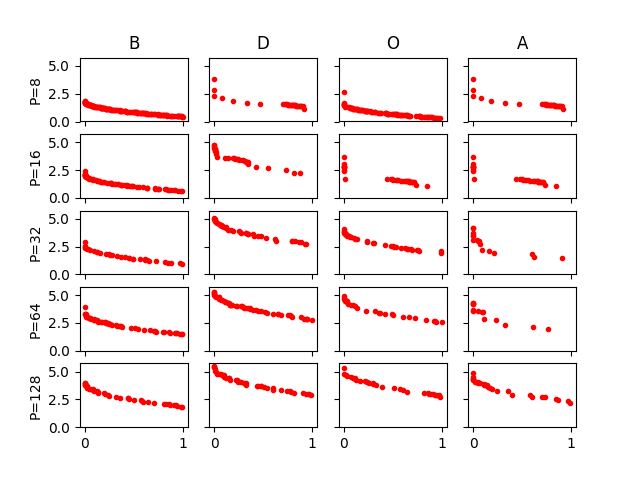
\includegraphics[width=12cm]{plot_zdt1_512.png}
\caption{\textcolor{blue}{PFs obtained in one arbitrary run for the ZDT1 problem with a chromosome size ($L$) of 512 for each combination of number of islands ($P$) and method: baseline ($B$), disjoint ($D$), overlapped ($O$) and automatic overlapped ($A$). Results for 8 and 16 islands of $A$ are equivalent of running $D$ and $O$ respectively. }}
\label{fig:plot_zdt1_512}
\end{figure}

\begin{figure}
\centering
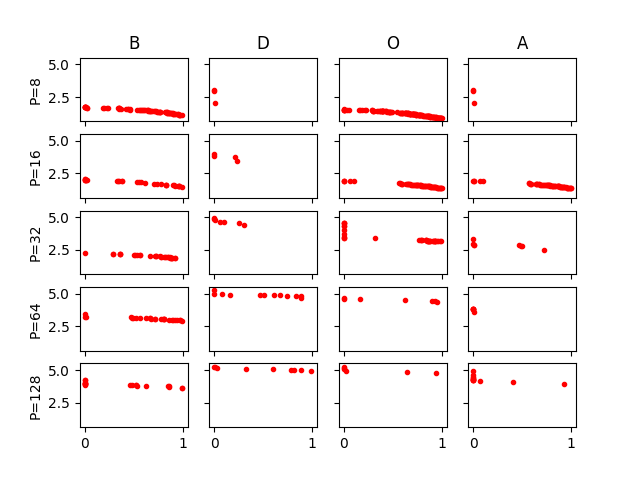
\includegraphics[width=12cm]{plot_zdt2_512.png}
\caption{\textcolor{blue}{PFs obtained in one arbitrary run for the ZDT2 problem with a chromosome size ($L$) of 512 for each combination of number of islands ($P$) and method: baseline ($B$), disjoint ($D$), overlapped ($O$) and automatic overlapped ($A$). Results for 8 and 16 islands of $A$ are equivalent of running $D$ and $O$ respectively. }}
\label{fig:plot_zdt2_512}
\end{figure}

\begin{figure}
\centering
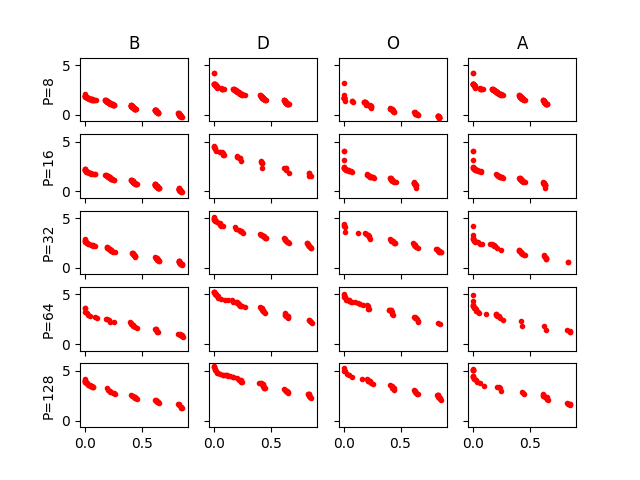
\includegraphics[width=12cm]{plot_zdt3_512.png}
\caption{\textcolor{blue}{PFs obtained in one arbitrary run for the ZDT3 problem with a chromosome size ($L$) of 512 for each combination of number of islands ($P$) and method: baseline ($B$), disjoint ($D$), overlapped ($O$) and automatic overlapped ($A$). Results for 8 and 16 islands of $A$ are equivalent of running $D$ and $O$ respectively. }}
\label{fig:plot_zdt3_512}
\end{figure}

\begin{figure}
\centering
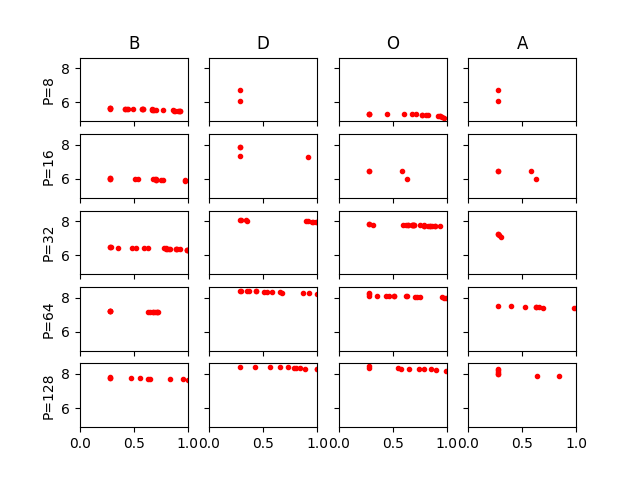
\includegraphics[width=12cm]{plot_zdt6_512.png}
\caption{\textcolor{blue}{PFs obtained in one arbitrary run for the ZDT6 problem with a chromosome size ($L$) of 512 for each combination of number of islands ($P$) and method: baseline ($B$), disjoint ($D$), overlapped ($O$) and automatic overlapped ($A$). Results for 8 and 16 islands of $A$ are equivalent of running $D$ and $O$ respectively. }}
\label{fig:plot_zdt6_512}
\end{figure}



%%%%%2018

\begin{figure}
\centering
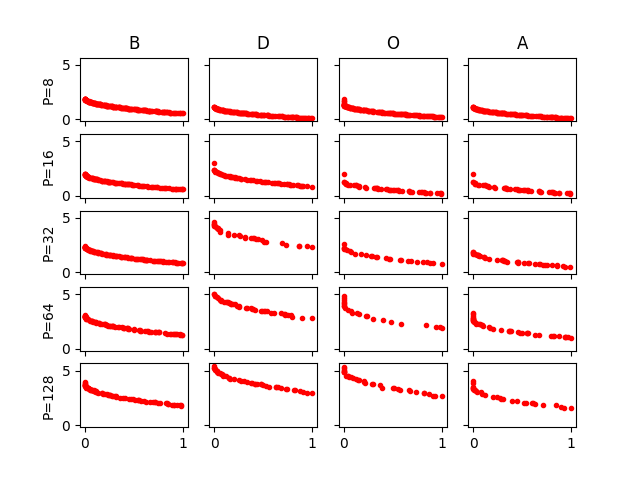
\includegraphics[width=12cm]{plot_zdt1_2048.png}
\caption{\textcolor{blue}{PFs obtained in one arbitrary run for the ZDT1 problem with a chromosome size ($L$) of 2048 for each combination of number of islands ($P$) and method: baseline ($B$), disjoint ($D$), overlapped ($O$) and automatic overlapped ($A$). Results for 8 and 16 islands of $A$ are equivalent of running $D$ and $O$ respectively. }}
\label{fig:plot_zdt1_2048}
\end{figure}

\begin{figure}
\centering
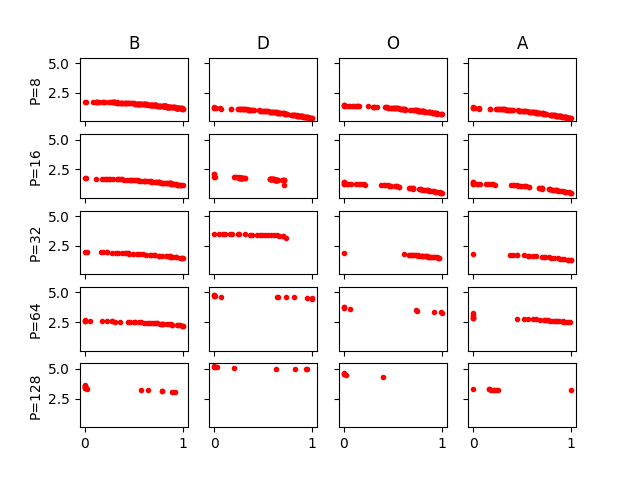
\includegraphics[width=12cm]{plot_zdt2_2048.png}
\caption{\textcolor{blue}{PFs obtained in one arbitrary run for the ZDT2 problem with a chromosome size ($L$) of 2048 for each combination of number of islands ($P$) and method: baseline ($B$), disjoint ($D$), overlapped ($O$) and automatic overlapped ($A$). Results for 8 and 16 islands of $A$ are equivalent of running $D$ and $O$ respectively. }}
\label{fig:plot_zdt2_2048}
\end{figure}

\begin{figure}
\centering
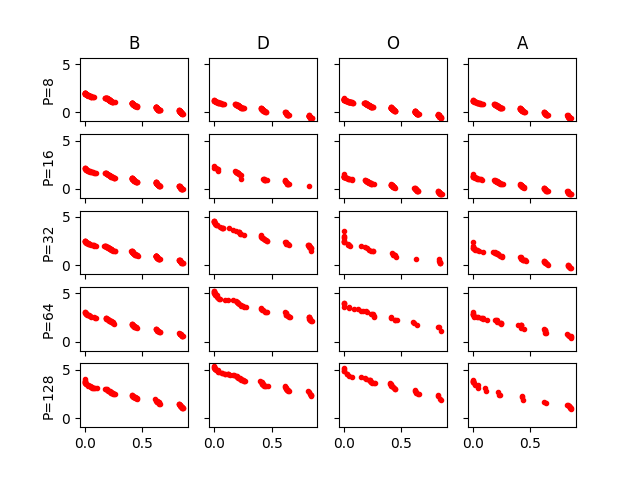
\includegraphics[width=12cm]{plot_zdt3_2048.png}
\caption{\textcolor{blue}{PFs obtained in one arbitrary run for the ZDT3 problem with a chromosome size ($L$) of 2048 for each combination of number of islands ($P$) and method: baseline ($B$), disjoint ($D$), overlapped ($O$) and automatic overlapped ($A$). Results for 8 and 16 islands of $A$ are equivalent of running $D$ and $O$ respectively. }}
\label{fig:plot_zdt3_2048}
\end{figure}

\begin{figure}
\centering
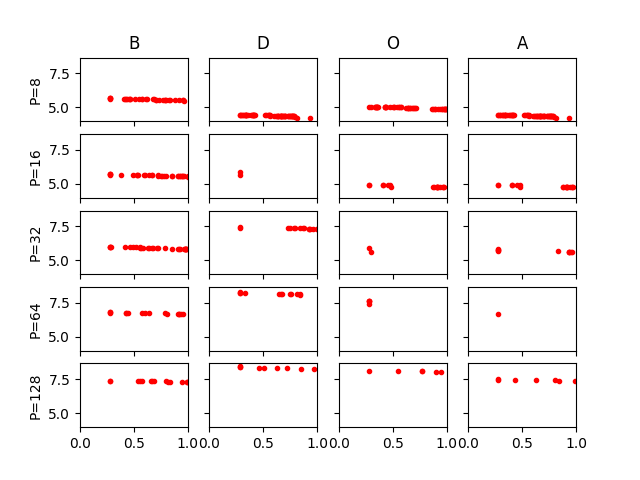
\includegraphics[width=12cm]{plot_zdt6_2048.png}
\caption{\textcolor{blue}{PFs obtained in one arbitrary run for the ZDT6 problem with a chromosome size ($L$) of 2048 for each combination of number of islands ($P$) and method: baseline ($B$), disjoint ($D$), overlapped ($O$) and automatic overlapped ($A$). Results for 8 and 16 islands of $A$ are equivalent of running $D$ and $O$ respectively. }}
\label{fig:plot_zdt6_2048}
\end{figure}



%EXPLANATION OF THE RESULTS
This can be explained comparing the number of non-dominated solutions
of each front and the average number of generations (Table
\ref{tab:sols512} and Table \ref{tab:sols2048}). With both chromosome
lengths, increasing the number of islands implies more generations
with all the methods (logically, as there are less individuals in each
island). But also, the SLA methods
approach to the number of generations with the baseline when
increasing the number of islands. However, with $L=2048$ the migration
time is big enough  to not improve the number of generations
with respect to the baseline, even in the lower number of islands, as
it happens with $L=512$. Therefore, more generations do not
necessarily improve the solution of the global PF, but focusing on
different elements of the chromosome. As  previously stated, every
island is unaware of the other islands PFs, and they are trying to
optimize their solutions independently. With respect to the average
number of solutions per front, there is a clear difference 
 with the baseline with $L=512$, where this value is in the most
of the cases, less than a half. The number of non-dominated solutions
also implies a better Spread indicator, where the baseline 
 obtains better (or not significantly different) values in the majority of the compared configurations. 

Finally, as it was already observed in \citep{Garcia16hpmoon}, results
show that all the quality indicators decrease in value when the number of islands is increased, as the  sizes of the subpopulations are smaller. This is consistent with the claim by Dorronsoro et al. \citep{Dorronsoro13superlinear}, who found that cooperative co-evolutionary MOEAs work better on bigger populations (more than 100 individuals).


%%%%REAL PROBLEM
%\subsection{Real problem benchmark: Unsupervised Feature Selection}
%\textcolor{red}{A real problem has also been used to BLABLABLA. In this case, the problem used to solve is the unsupervised feature selection. A dataset formed by EEG signals from Brain Computer Interface (BCI) is used as a benchmark \cite{Kimovski15Parallel}, due to the required high computational cost and chromosome length. Individuals in this case are binary vectors indicating if a specific feature is selected or not. To evaluate a set of features different clustering validation indexes (CVIs) can be used.}

%\textcolor{red}{In this case, the two objectives to compare the three methods are the inter-cluster separation ($f1$) and the intra-cluster separation ($f2$). To obtain this measures, and after applying the projection to the dataset, a method based in the one presented  \cite{Kimovski15Parallel} is applied. Starting with a random value of the projection, the distance to the closer one is stored, and so on. After ordering these distances from lower to higher, we consider the intra-cluster distance ($f1$) as the one in the position 1/4 of the list, while the inter-cluster ($f2$) distance is in the position 3/4. The intra-cluster distance objective needs to be minimized, while the inter-cluster is maximized. Figure \ref{fig:cvis} explains this method using a extremely simplified example. Note that the goal of this paper is not obtain better CVI values than other methods, but to study the different overlapping schemes in parallel MOEAs.}

%\begin{figure}
%\centering
%\includegraphics[width=10cm]{clusterCVI.pdf}
%\caption{\textcolor{red}{Method to calculate the two objectives for the Feature Selection problem. Starting from a random $d$ point of the projection of the features, the distance to the closer point is calculated iteratively. After ordering these distances, the one in the position 1/4 (a) is considered the intra-cluster distance, while the one in position 3/4 (b) is considered the inter-cluster one.}}
%\label{fig:cvis}
%\end{figure}


%\textcolor{red}{The Dataset used is ... Due to the high computational cost required for the fitness function, the running time for each run has been set to 4 hours, with two generations before sending the individual to another random island. Table \ref{tab:parametersBCI} summarizes the specific parameters for this experiment (the rest of the parameters are the same than the previous experiment, shown in Table \ref{tab:parameters} ). As there is no optimal PF known for this problem, we have used the paretos obtained from all runs to obtain the optimal PF to apply the IGD quality metric.}

%\textcolor{red}{
%\begin{table*}
%\begin{center}
%\begin{tabular}{|c|c|}
%\hline
%{\em Parameter Name} & {\em Value} \\ \hline
%Number of islands ($P$) & 8, 32 and 128 \\ \hline
%Chromosome size ($L$) & 3600 \\ \hline
%Crossover type & One-point \\ \hline
%Mutation  type & flip\\ \hline
%Generations between migration & 2 \\ \hline
%Runs per configuration & 10 \\ \hline
%\end{tabular}
%\caption{\textcolor{red}{Parameters and operators used in the experiments for Feature Selection problem (the rest of the parameters are the ones described in Table \ref{tab:parameters}).}}
%\label{tab:parametersBCI}
%\end{center}
%\end{table*}
%}






\section{Conclusions}

Problems that require high-performance % problems are not high-performance. They
                          % _require_ high performance Fergu: done
 and deal with a large number of decision variables can leverage the
 division of the decision space that parallel and distributed
 algorithms imply. This can be done in dMOEAs by selective operator application (SLA), that is, dividing the
 chromosome into different parts, each one modified by a different
 island. This paper compares a baseline distributed NSGA-II with three
 different strategies to separate the chromosome (disjoint or
 overlapping parts), using a high number of islands. Results show that
 these methods can achieve better quality metrics than the baseline in
 the same amount of time, with large chromosome lengths. 

Obtained results also show that when increasing the number of islands, the
automatic overlapping method ($A$) significantly improves the results with
respect to the disjoint and overlapped methods. However, this is only
apparent with larger chromosome sizes. Therefore, the length of the
chromosome is also a key factor to take into account in automatic overlapping
methods, and not only the number of islands. Studying this factor with
more types of problems, and new configurations of population size and
chromosome lengths could be addressed in the future. \textcolor{blue}{Since our method divides the individuals into blocks of divisible size, aggregation methods after migration, such as the ones used in \cite{Kimovski15Parallel} or \cite{Dorronsoro13superlinear} can be also tested. But as we are dealing with complete individuals in each island, the possibility of using a real number, such as 0.3 (30\% overlapping) instead an integer value opens future experimental setups.}
For example, comparing 
different ways to calculate $c$ using linear, logarithmic or exponential functions
depending \textcolor{blue}{on population size, number of islands, or other values}. Moreover, a diversity analysis of the individuals
in each island during the algorithm run could be carried out to understand its influence
on results.
% 
% More discussion should be added. Why is adaptive better? Is the high
% performance really needed? - JJ
% STILL more discussion should be needed. For instance, the last
% paragraph of results begs an explanation of the influence of diversity on
% results - JJ Pablo: extending this section

Also, more distributed implementations in several systems (such as a
GPUs or heterogeneous clusters) with different amounts of
islands/processors, could be used to perform a scalability study of the
different methods, being the transmission time between islands a
relevant issue to be addressed. Other MOEA algorithms available in the literature, such as SPEA or MOEA/D could be compared. Finally, new benchmarks and real problems
could also be  used to validate this approach.  



\section*{Acknowledgements}
This work has been partially funded by projects TIN2014-56494-C4-3-P, TIN2015-67020-P and TIN2017-85727-C4-2-P (Spanish Ministry of Economy and Competitiveness and FEDER).



\section*{References}

\bibliographystyle{elsarticle-num}
\bibliography{hpmoon-asoco}



\end{document}
